\documentclass[UTF8,aspectratio=169,11pt]{ctexbeamer}

\usetheme{Madrid}
\usecolortheme{seahorse}
\usefonttheme{professionalfonts}

\usepackage{amsmath}
\usepackage{amssymb}
\usepackage{graphicx}
\usepackage{booktabs}
\usepackage{array}
\usepackage{tabularx}
\usepackage{tikz}
\usetikzlibrary{positioning,arrows.meta,fit}

\hypersetup{colorlinks=true,linkcolor=black,urlcolor=blue}
\setbeamertemplate{navigation symbols}{}
\setbeamertemplate{caption}[numbered]
\setbeamertemplate{footline}[frame number]

\definecolor{lorenzblue}{RGB}{35,83,135}
\definecolor{lorenzteal}{RGB}{27,124,117}
\definecolor{lorenzorange}{RGB}{205,104,38}
\definecolor{lorenzgray}{RGB}{80,86,94}
\setbeamercolor{title}{fg=lorenzblue}
\setbeamercolor{frametitle}{fg=lorenzblue}
\setbeamercolor{structure}{fg=lorenzteal}

\newcommand{\xvec}{\mathbf{x}}
\newcommand{\Xwin}{\mathbf{X}}
\newcommand{\dt}{\Delta t}
\newcommand{\crmse}{\mathrm{CRMSE}}
\newcommand{\mse}{\mathrm{MSE}}

\title[高维混沌长期预测]{基于 MATLAB 的高维混沌系统长期预测建模}
\subtitle{Lorenz-63 铺垫与 Lorenz-96 10D Ultimate Hybrid}
\author{钟兴涛 \quad 唐亦明 \quad 戴云天 \quad 任宇航 \quad 黄宇轩}
\institute{MATLAB及应用（强）}
\date{\today}

\begin{document}

\begin{frame}
    \titlepage
\end{frame}

\begin{frame}{汇报主线}
    \tableofcontents
\end{frame}

\section{问题动机}

\begin{frame}{真正的问题不是 one-step，而是 rollout}
    \small
    \begin{columns}[T,onlytextwidth]
        \begin{column}{0.50\textwidth}
            \begin{block}{单步预测看起来容易}
                \begin{itemize}
                    \item 输入真实历史状态；
                    \item 预测下一步或短 horizon；
                    \item 测试分布接近训练分布。
                \end{itemize}
            \end{block}
            \begin{alertblock}{长期推演才是难点}
                \begin{itemize}
                    \item 后续输入来自模型自己的预测；
                    \item 小误差被混沌动力学放大；
                    \item 轨迹逐渐偏离真实吸引子附近。
                \end{itemize}
            \end{alertblock}
        \end{column}
        \begin{column}{0.46\textwidth}
            \centering
            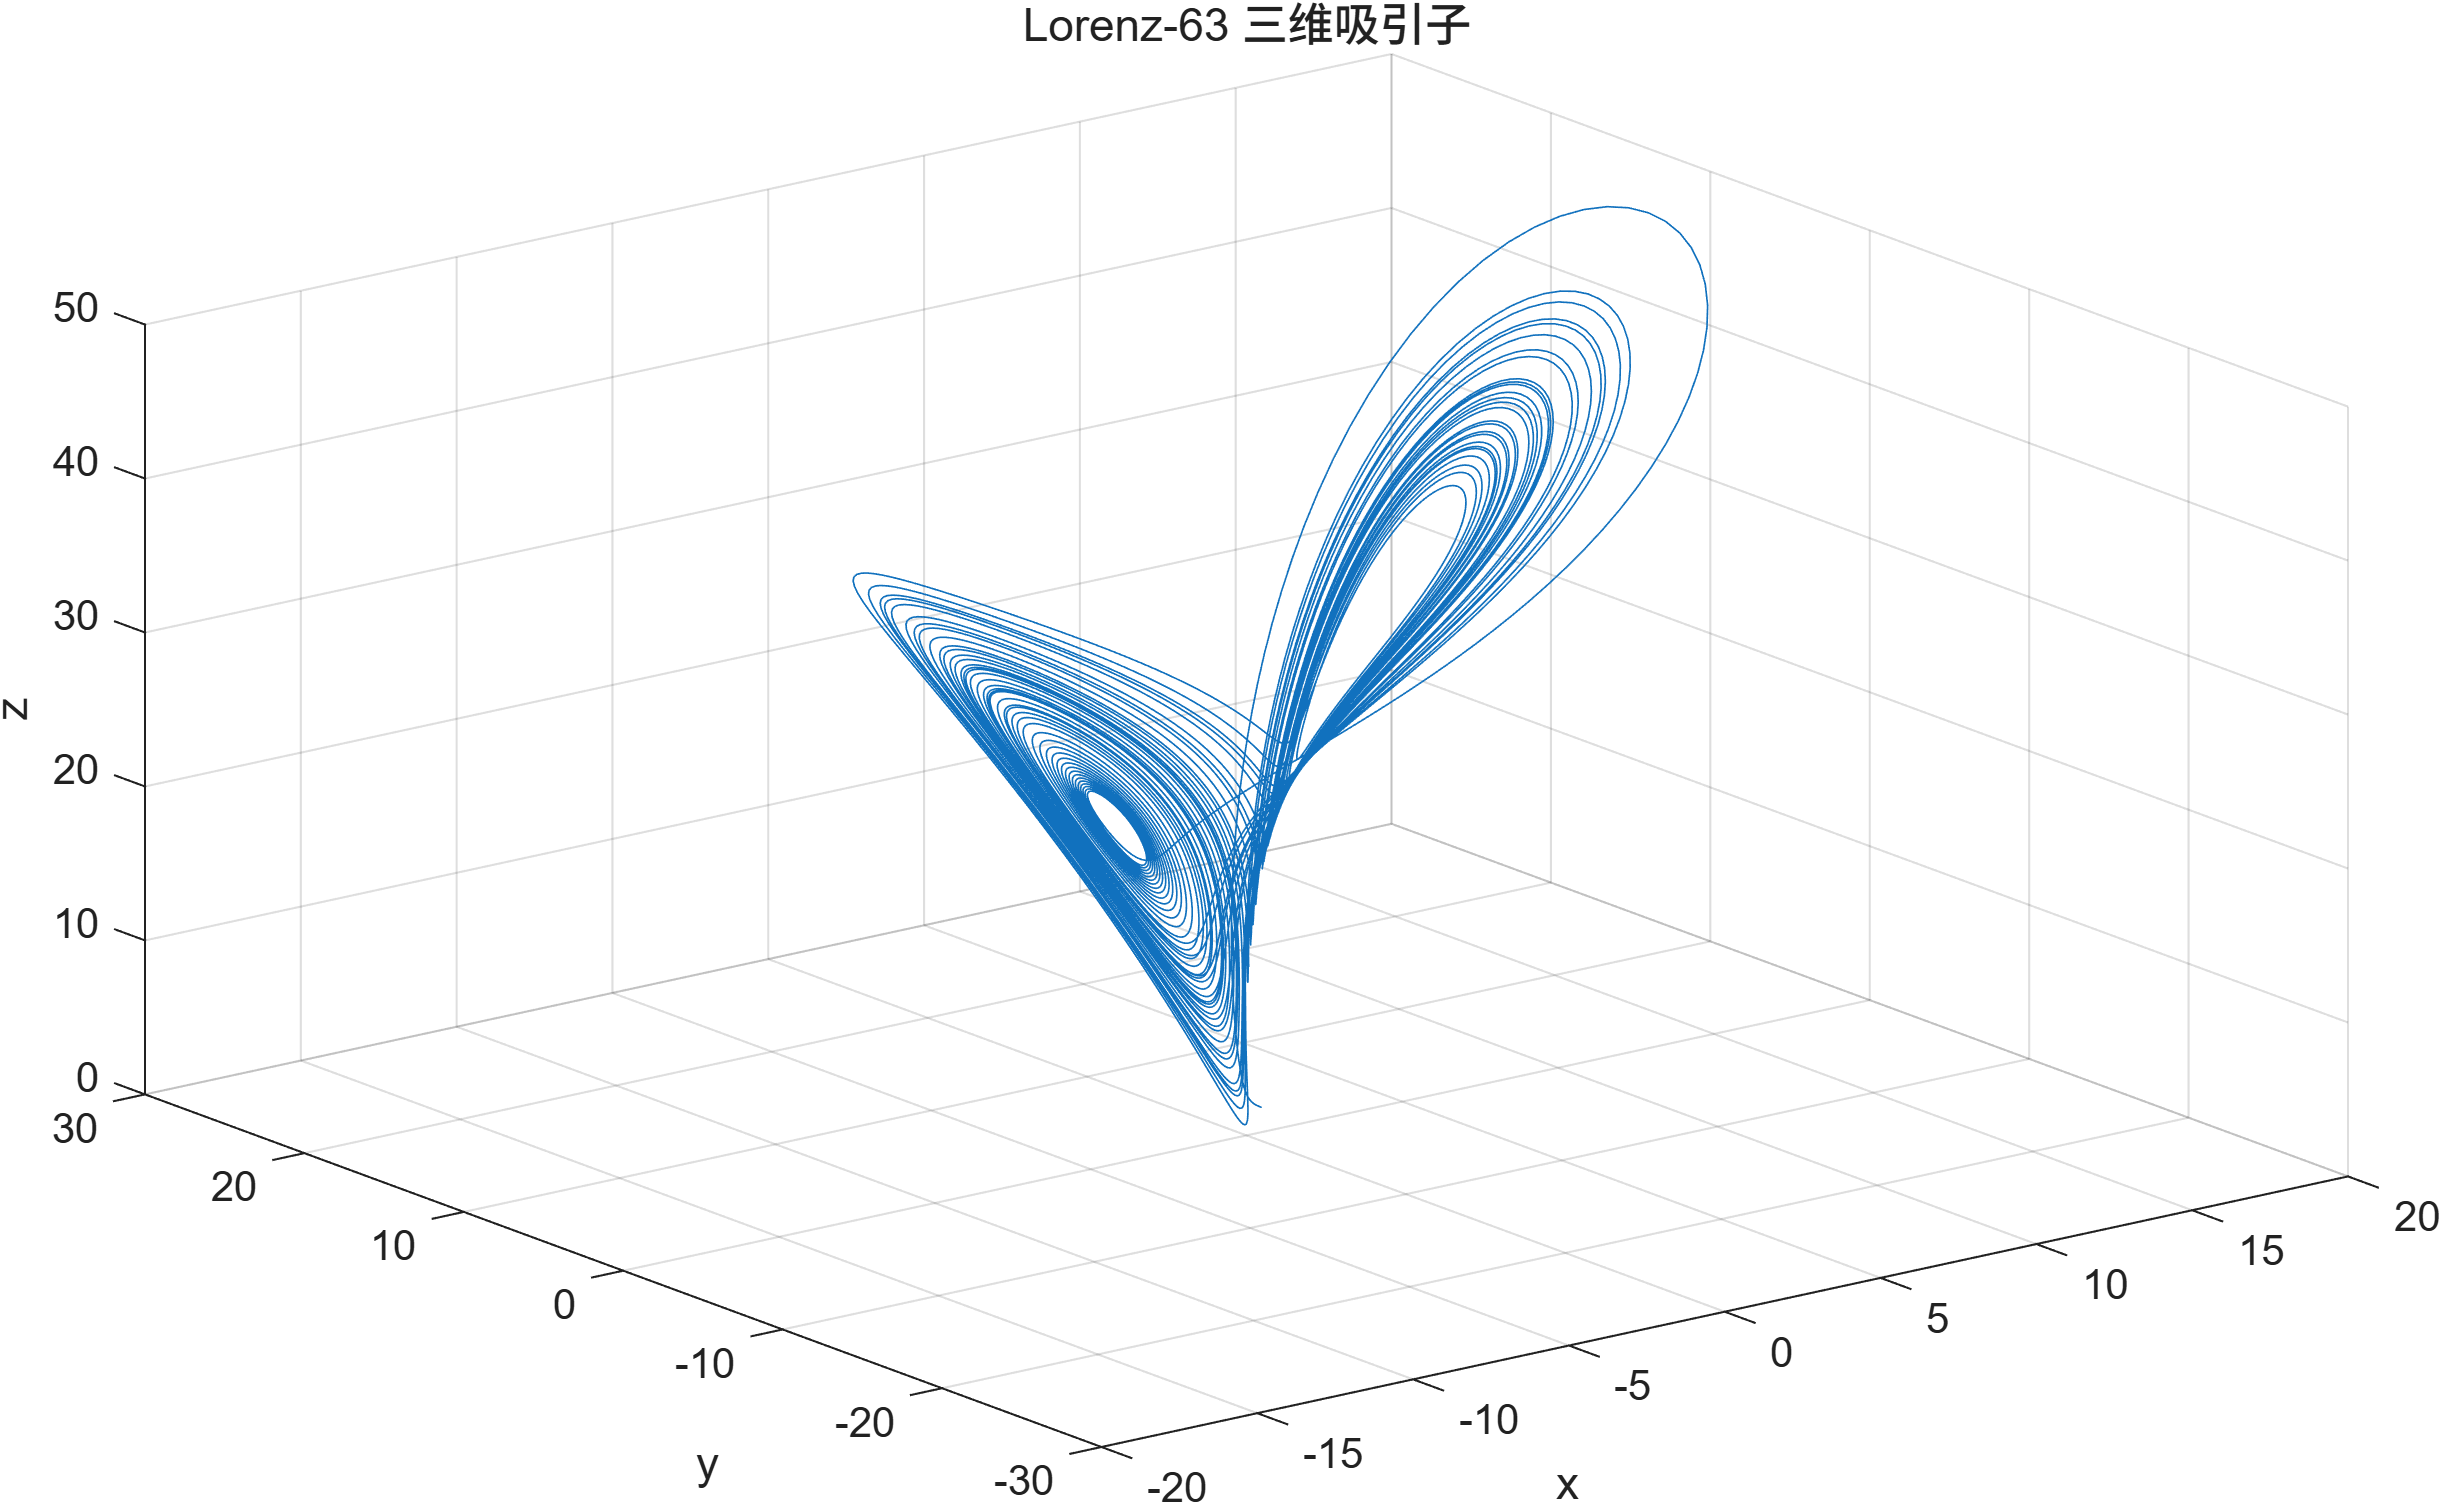
\includegraphics[width=0.84\linewidth]{figures/lorenz_attractor.png}
            \vspace{0.2em}
            {\small Lorenz 吸引子：短期连续，长期敏感}
        \end{column}
    \end{columns}
\end{frame}

\begin{frame}{Lorenz-63：基础模型可以短期拟合，但 rollout 会发散}
    \small
    \begin{columns}[T,onlytextwidth]
        \begin{column}{0.45\textwidth}
            \begin{table}
                \centering
                \scriptsize
                \begin{tabular}{lcc}
                    \toprule
                    模型 & 短期 RMSE & 500-step RMSE \\
                    \midrule
                    Linear Reg. & 0.5383 & 17.2665 \\
                    Random Forest & 0.0913 & 1.7883 \\
                    MLP & 0.0138 & 6.6833 \\
                    \bottomrule
                \end{tabular}
            \end{table}
            \begin{block}{启示}
                Lorenz-63 证明：短期局部映射可学，但不能说明长期轨迹稳定。
            \end{block}
        \end{column}
        \begin{column}{0.52\textwidth}
            \centering
            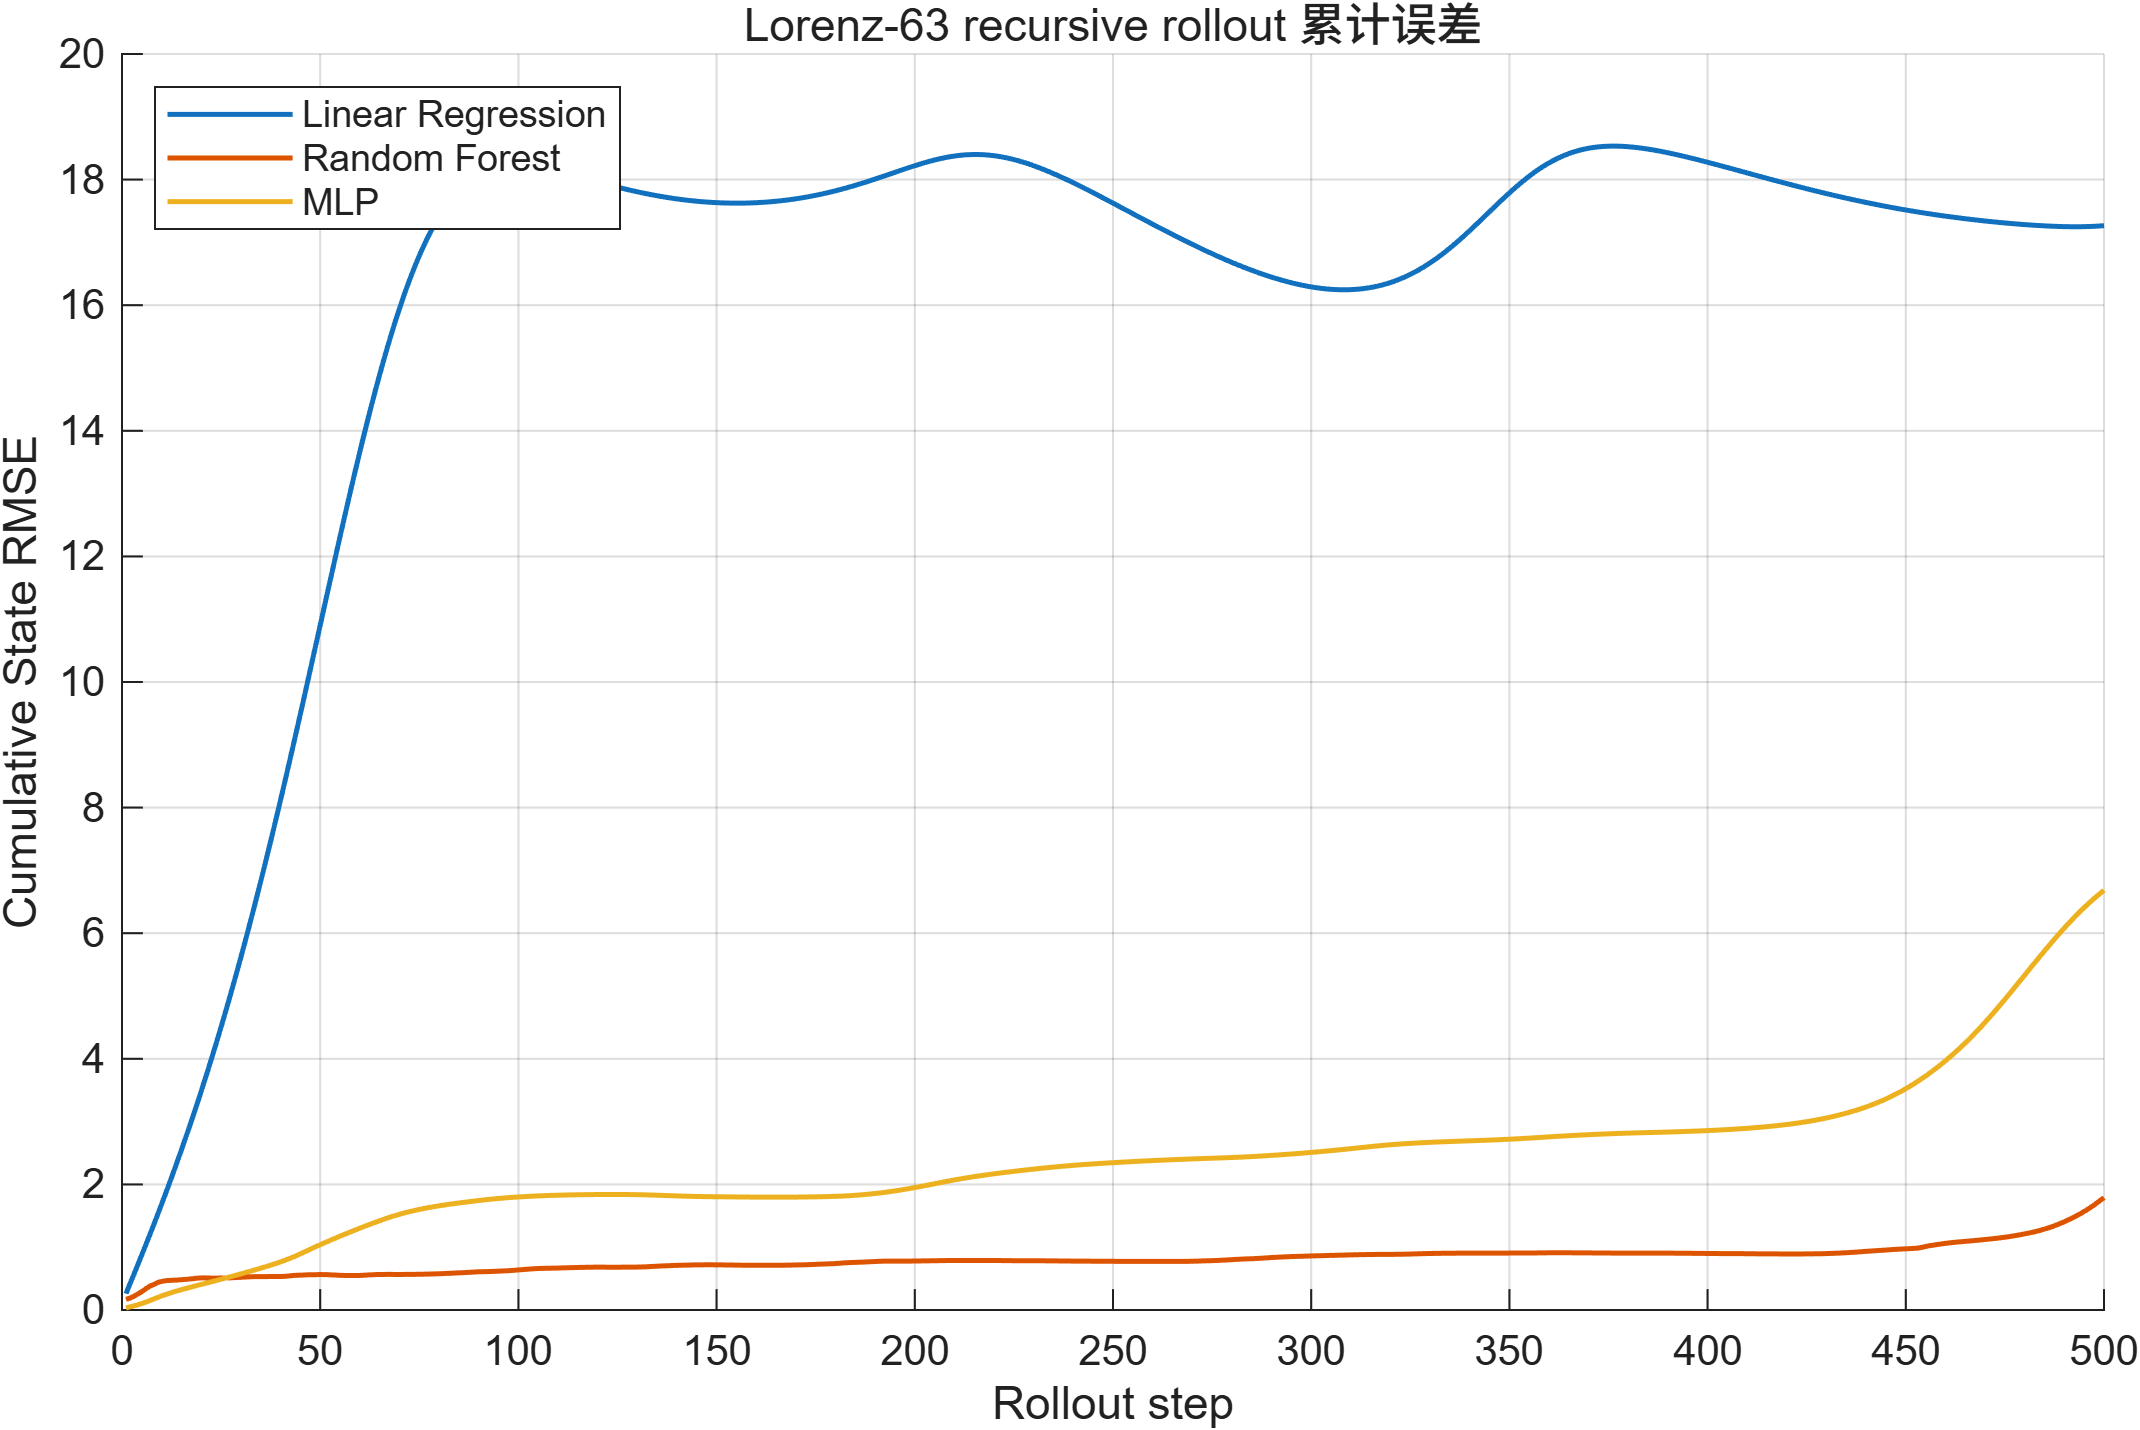
\includegraphics[width=\linewidth]{figures/rollout_error.png}
            {\small 基础模型 recursive rollout 误差累积}
        \end{column}
    \end{columns}
\end{frame}

\begin{frame}[shrink=15]{数据构建与可视化检查}
    \scriptsize
    \begin{block}{数据与预处理}
        数值积分生成状态序列；按时间顺序切分训练/测试集；检查缺失值，并用训练集统计量进行 z-score 标准化。
    \end{block}
    \vspace{-0.4em}
    \begin{columns}[T,onlytextwidth]
        \begin{column}{0.48\textwidth}
            \centering
            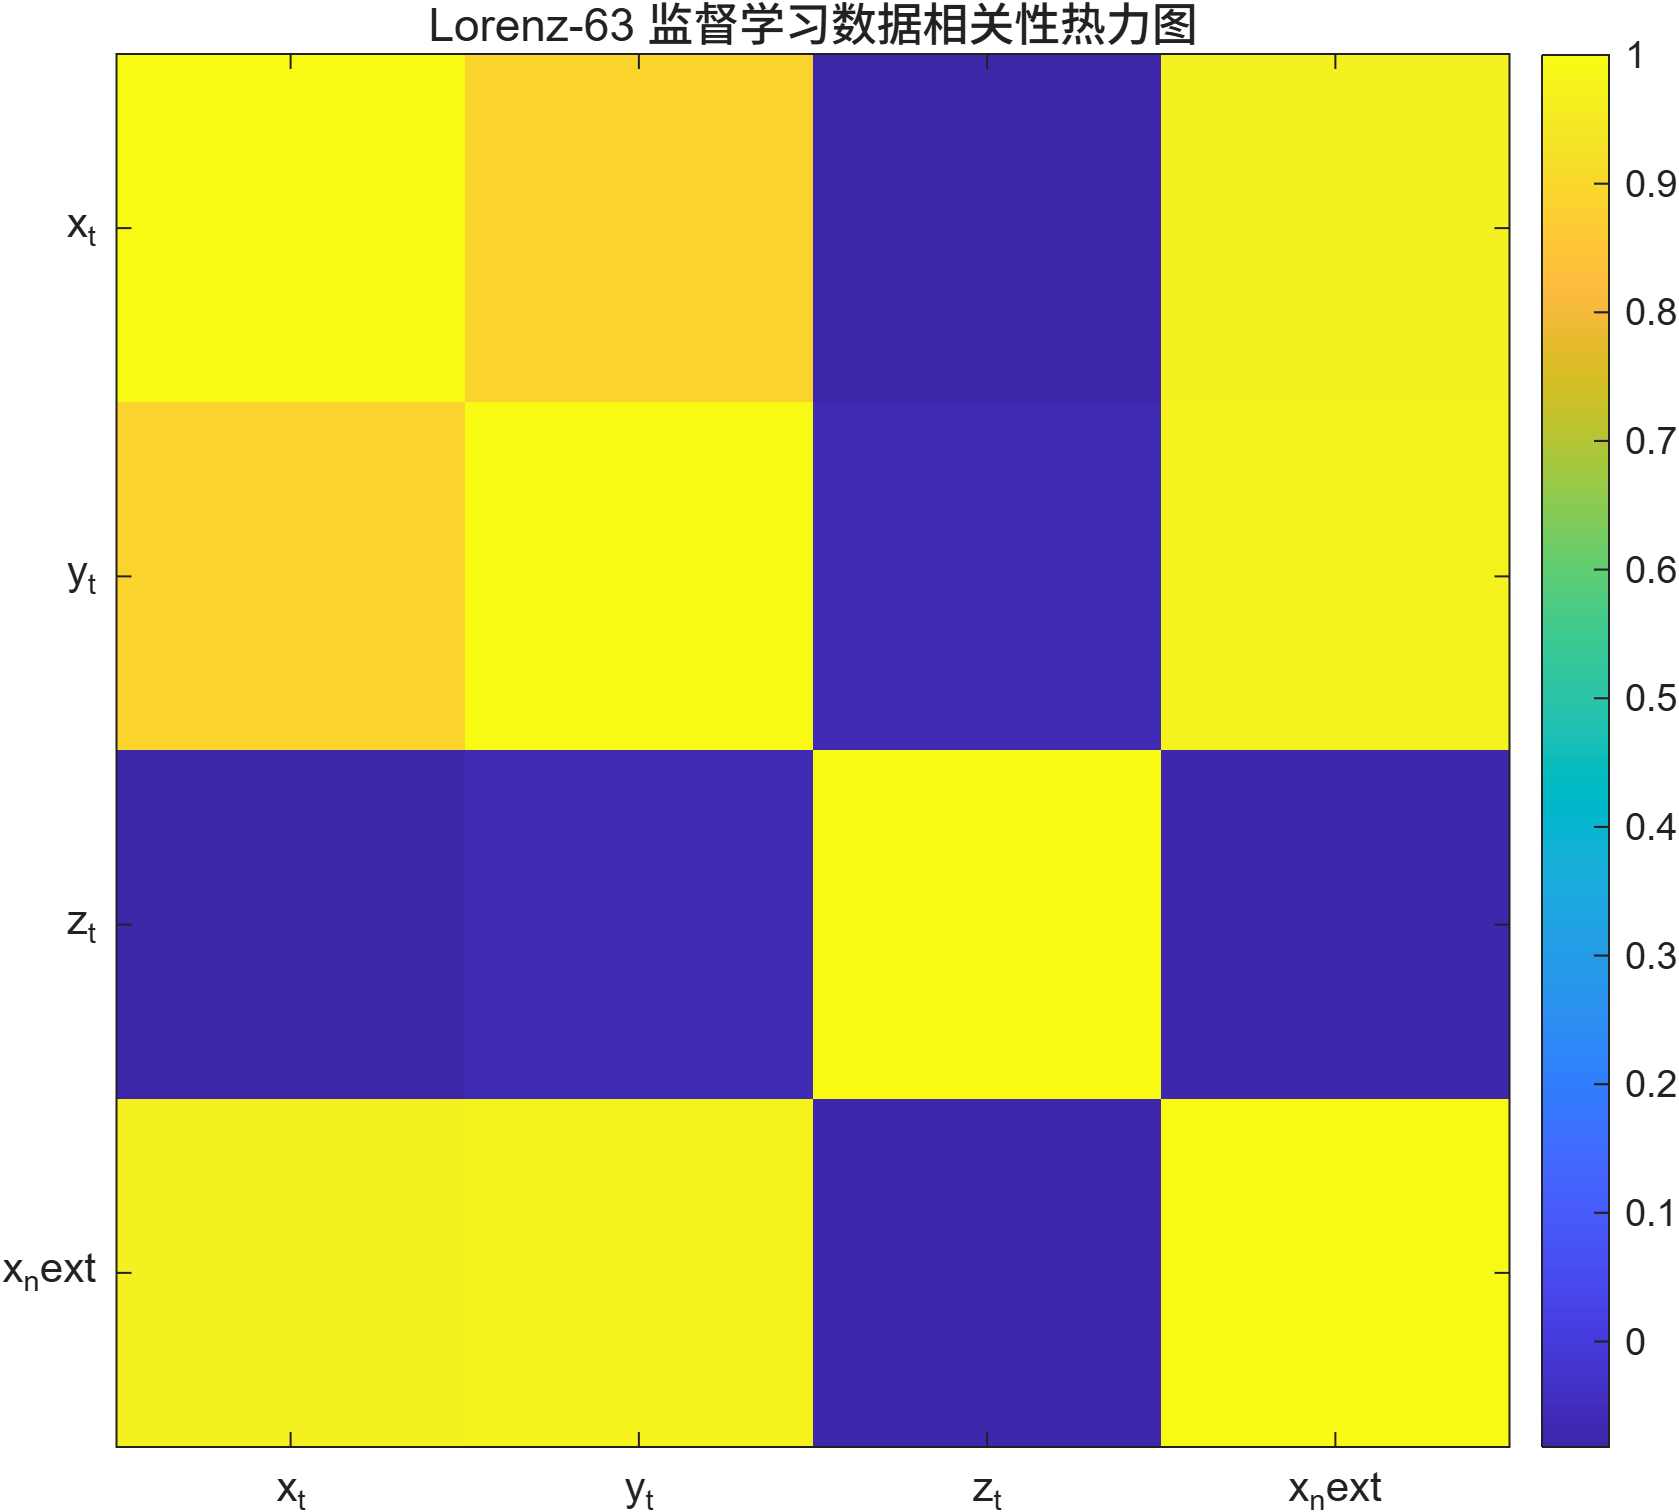
\includegraphics[width=0.66\linewidth]{figures/correlation_heatmap.png}
            {\scriptsize 相关性热力图：验证短期局部状态可学习}
        \end{column}
        \begin{column}{0.48\textwidth}
            \centering
            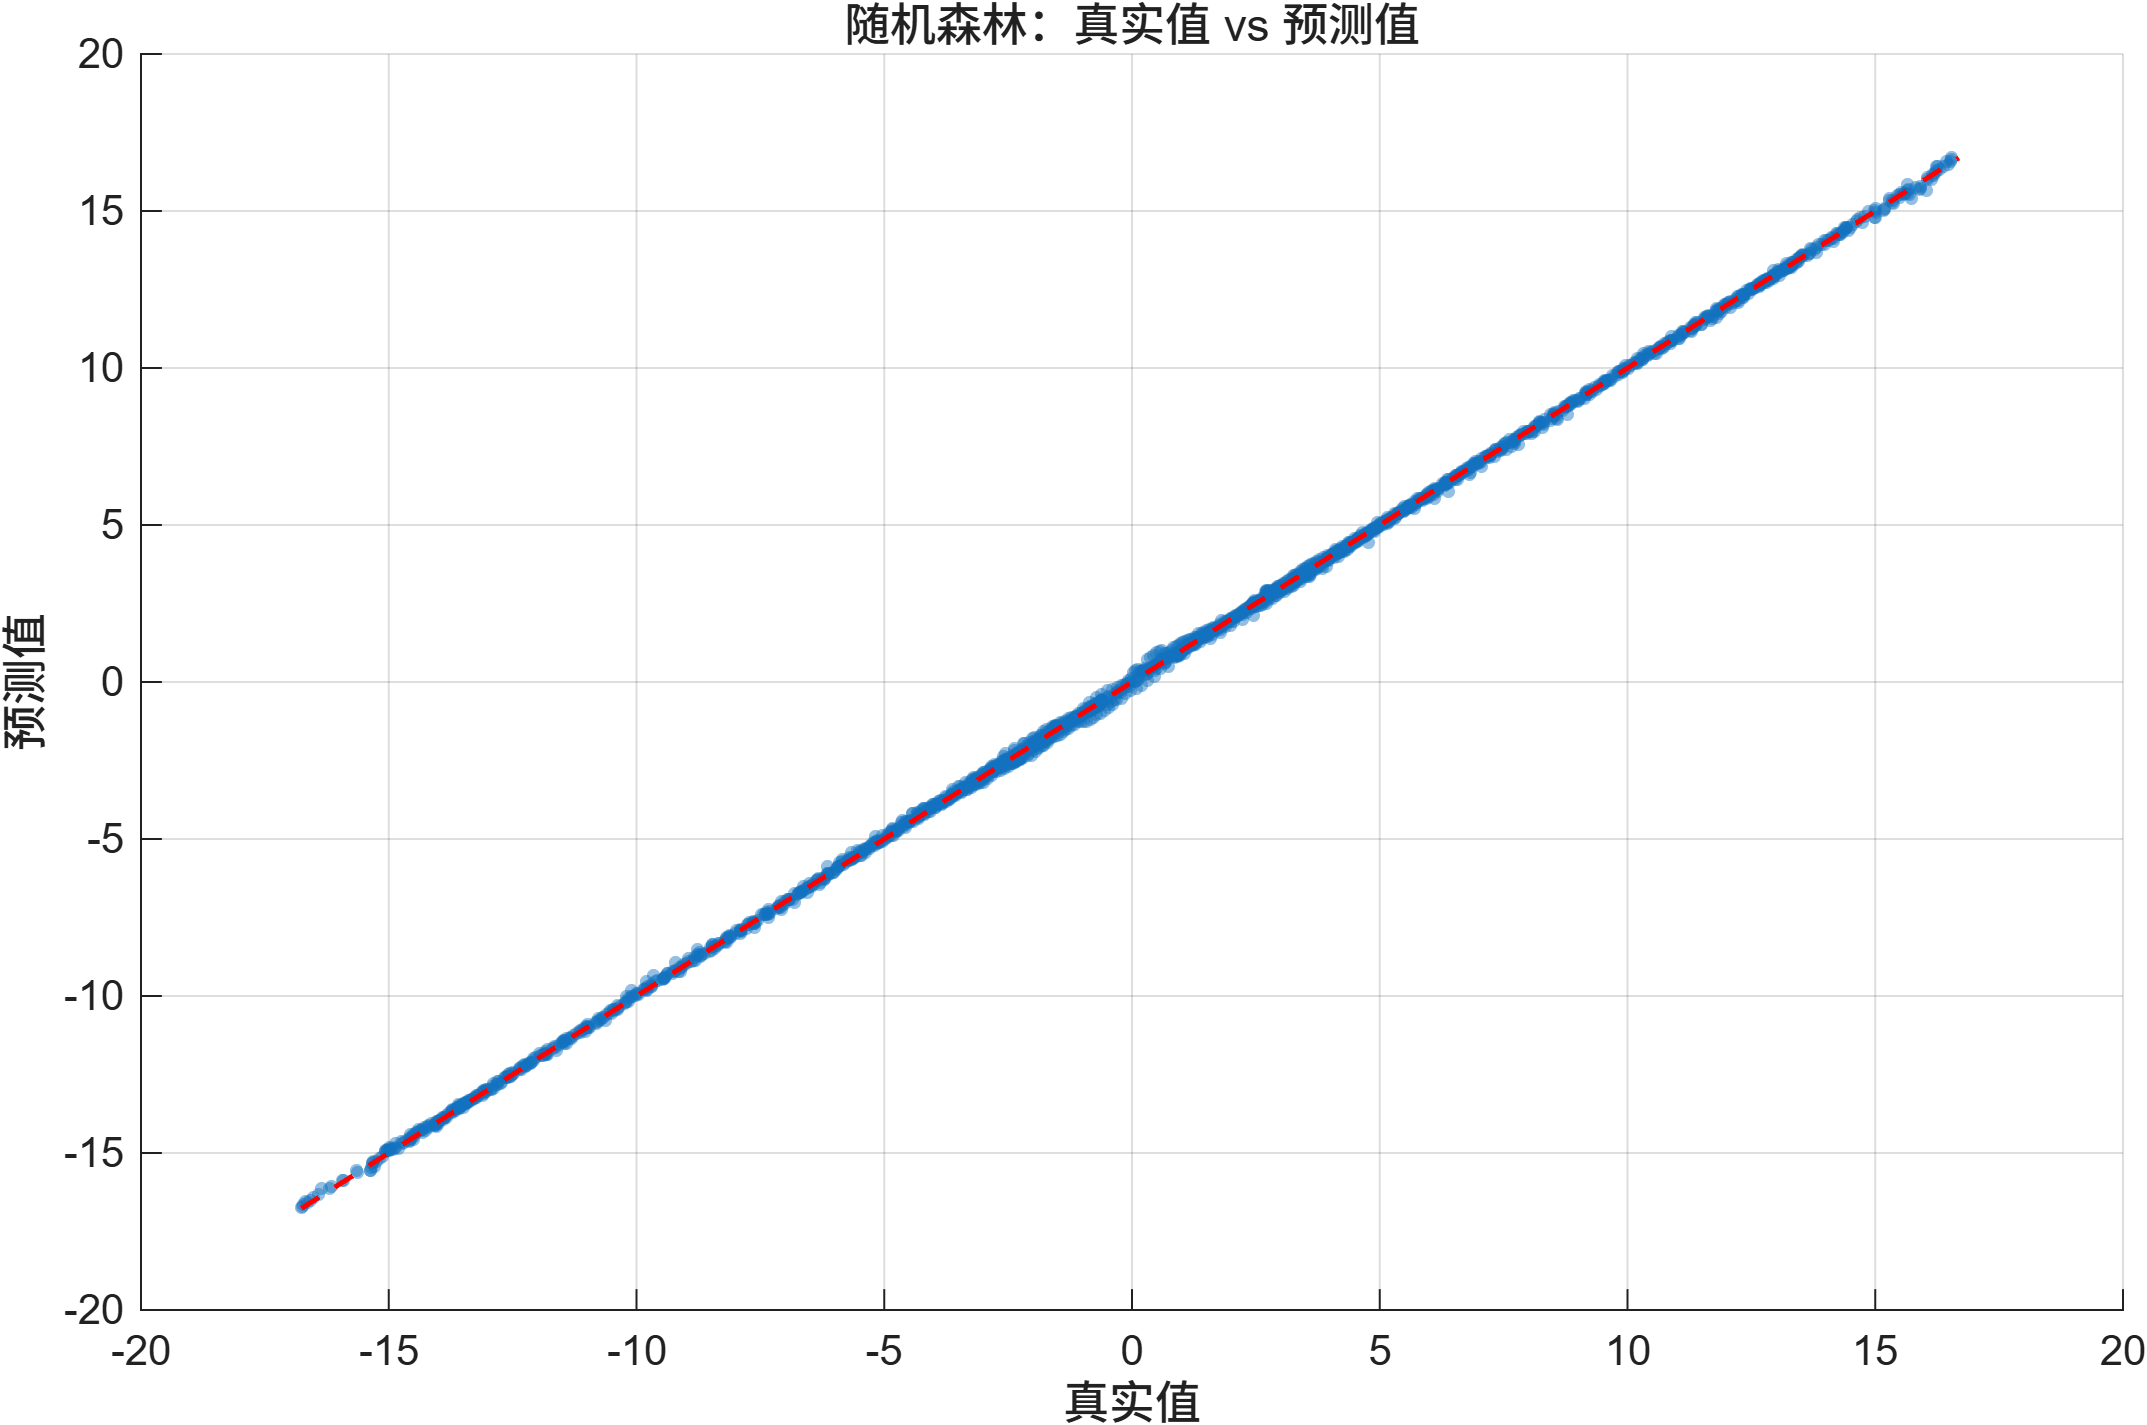
\includegraphics[width=0.66\linewidth]{figures/prediction_scatter_rf.png}
            {\scriptsize 真实值 vs. 预测值：极端状态下偏差更明显}
        \end{column}
    \end{columns}
    \vspace{-0.2em}
    \begin{alertblock}{汇报时强调}
        散点图说明短期拟合较好，但长期能力必须用 500-step rollout 单独评价。
    \end{alertblock}
\end{frame}

\begin{frame}{转向核心任务：Lorenz-96 10D 长期多步预测}
    \begin{block}{Lorenz-96 动力学}
        \[
        \frac{dx_i}{dt}=(x_{i+1}-x_{i-2})x_{i-1}-x_i+F,\quad i=1,\dots,N
        \]
        \[
        x_{i+N}=x_i,\qquad N=10,\qquad F_{\mathrm{true}}=8.0
        \]
    \end{block}
    \begin{columns}[T,onlytextwidth]
        \begin{column}{0.48\textwidth}
            \begin{itemize}
                \item 变量维度更高，耦合关系更复杂；
                \item 周期边界使每个变量依赖邻近状态；
                \item 500-step rollout 更能暴露长期稳定性。
            \end{itemize}
        \end{column}
        \begin{column}{0.48\textwidth}
            \begin{alertblock}{本文核心问题}
                如何设计一个兼顾物理结构、历史窗口特征和 rollout 稳定性的模型？
            \end{alertblock}
        \end{column}
    \end{columns}
\end{frame}

\section{多步预测定义}

\begin{frame}{窗口序列预测}
    \begin{block}{历史窗口}
        \[
        \Xwin_t=(\xvec_{t-w+1},\xvec_{t-w+2},\dots,\xvec_t)\in \mathbb{R}^{w\times N}
        \]
    \end{block}
    \begin{block}{One-step prediction}
        \[
        \hat{\xvec}_{t+1}=f_\theta(\Xwin_t)
        \]
    \end{block}
    \begin{alertblock}{问题}
        One-step evaluation 使用真实窗口；rollout evaluation 会不断把模型预测拼回窗口。
    \end{alertblock}
\end{frame}

\begin{frame}{Recursive rollout 与累计 RMSE}
    \begin{align*}
    \hat{\xvec}_{t+1} &= f_\theta(\xvec_{t-w+1},\dots,\xvec_t),\\
    \hat{\xvec}_{t+2} &= f_\theta(\xvec_{t-w+2},\dots,\xvec_t,\hat{\xvec}_{t+1}),\\
    \hat{\xvec}_{t+m} &= f_\theta(\hat{\xvec}_{t+m-w},\dots,\hat{\xvec}_{t+m-1}).
    \end{align*}
    \vspace{-0.3em}
    \begin{block}{500-step 累计 RMSE}
        \[
        \crmse(T)=
        \sqrt{
        \frac{1}{T}\sum_{m=1}^{T}
        \left\|\xvec_{t+m}-\hat{\xvec}_{t+m}\right\|_2^2
        },\quad T=500
        \]
    \end{block}
    \begin{alertblock}{评价重点}
        本文不只看 one-step RMSE，而以 500-step $\crmse$ 衡量长期推演稳定性。
    \end{alertblock}
\end{frame}

\section{模型演进}

\begin{frame}{第一步：Baseline LSTM 到 Residual LSTM}
    \begin{columns}[T,onlytextwidth]
        \begin{column}{0.48\textwidth}
            \begin{block}{直接预测}
                \[
                \hat{\xvec}_{t+1}=f_{\theta}^{\mathrm{LSTM}}(\Xwin_t)
                \]
            \end{block}
            \begin{block}{残差预测}
                \[
                \Delta\hat{\xvec}_{t+1}=g_{\theta}^{\mathrm{LSTM}}(\Xwin_t)
                \]
                \[
                \hat{\xvec}_{t+1}=\xvec_t+\Delta\hat{\xvec}_{t+1}
                \]
            \end{block}
        \end{column}
        \begin{column}{0.48\textwidth}
            \begin{itemize}
                \item 连续动力系统相邻状态变化较小；
                \item 学习增量比学习绝对状态更容易；
                \item 加入 LayerNorm 与 gradient clipping 提升训练稳定性。
            \end{itemize}
            \begin{alertblock}{核心直觉}
                残差学习让模型更像一个数据驱动的局部积分器。
            \end{alertblock}
        \end{column}
    \end{columns}
\end{frame}

\begin{frame}{第二步：Scheduled Sampling 缓解分布偏移}
    \begin{columns}[T,onlytextwidth]
        \begin{column}{0.52\textwidth}
            \begin{block}{训练时多步展开}
                \[
                \mathcal{L}_{multi}=
                \frac{1}{M}\sum_{m=1}^{M}
                \mse(\hat{\xvec}_{t+m},\xvec_{t+m}),\quad M=5
                \]
            \end{block}
            \begin{block}{Refined inverse-sigmoid schedule}
                \[
                p_e=\frac{k}{k+\exp(e/(E/10))}
                \]
            \end{block}
        \end{column}
        \begin{column}{0.44\textwidth}
            \begin{itemize}
                \item 以概率 $p_e$ 使用真实状态；
                \item 以概率 $1-p_e$ 使用模型预测；
                \item 训练阶段更接近 rollout 环境。
            \end{itemize}
            \begin{alertblock}{注意}
                Scheduled sampling 不是总能改善结果，衰减策略和多步展开方式很关键。
            \end{alertblock}
        \end{column}
    \end{columns}
\end{frame}

\begin{frame}{第三步：PINN 物理约束}
    \begin{block}{Lorenz-96 向量场}
        \[
        \mathbf{f}_{L96}(\xvec;F)=
        \left((x_{i+1}-x_{i-2})x_{i-1}-x_i+F\right)_{i=1}^{N}
        \]
    \end{block}
    \begin{block}{有限差分导数与物理导数对齐}
        \[
        \mathcal{L}_{phys}=
        \left\|
        \frac{\hat{\xvec}_{t+1}-\xvec_t}{\dt}
        -
        \mathbf{f}_{L96}(\xvec_t;F_{\mathrm{true}})
        \right\|_2^2
        \]
    \end{block}
    \begin{block}{总损失}
        \[
        \mathcal{L}=\mathcal{L}_{data}+0.1\mathcal{L}_{phys}
        \]
    \end{block}
\end{frame}

\begin{frame}{第四步：Transformer 捕捉历史窗口关系}
    \begin{columns}[T,onlytextwidth]
        \begin{column}{0.50\textwidth}
            \begin{align*}
            \mathbf{Z}_t &= \mathrm{PE}(\mathrm{Linear}(\Xwin_t)),\\
            \mathbf{H}_t &= \mathrm{TransformerEncoder}(\mathbf{Z}_t),\\
            \Delta\hat{\xvec}_{t+1} &= W\mathbf{H}_{t,-1}+b.
            \end{align*}
        \end{column}
        \begin{column}{0.46\textwidth}
            \begin{itemize}
                \item LSTM 用单个隐藏状态压缩历史；
                \item Transformer 通过 self-attention 建立窗口内时间步关联；
                \item 更适合捕捉高维相空间中的局部演化趋势。
            \end{itemize}
        \end{column}
    \end{columns}
\end{frame}

\begin{frame}{第五步：不完美物理求解器 + 残差学习}
    \begin{block}{不完美物理基底}
        \[
        F_{\mathrm{true}}=8.0,\qquad F_{\mathrm{imp}}=8.5
        \]
        \[
        \xvec^{phys}_{t+1}=\Phi_{\dt}^{F_{\mathrm{imp}}}(\xvec_t)
        \]
    \end{block}
    \begin{block}{Hybrid prediction}
        \[
        \hat{\xvec}_{t+1}
        =
        \xvec^{phys}_{t+1}
        +
        g_\theta(\Xwin_t)
        \]
    \end{block}
    \begin{alertblock}{设计思想}
        物理求解器负责主要动力学演化，神经网络只学习参数偏差和模型误差导致的残差。
    \end{alertblock}
\end{frame}

\begin{frame}{Ultimate Hybrid：最终架构}
    \centering
    \begin{tikzpicture}[
        node distance=0.65cm,
        box/.style={rounded corners, draw=lorenzblue, thick, align=center, minimum width=3.0cm, minimum height=0.72cm, fill=blue!5},
        core/.style={rounded corners, draw=lorenzorange, thick, align=center, minimum width=3.1cm, minimum height=0.76cm, fill=orange!10},
        arrow/.style={-{Latex[length=2mm]}, thick, draw=lorenzgray}
    ]
        \node[box] (hist) {历史窗口\\$\xvec_{t-w+1:t}$};
        \node[core, below left=0.85cm and 1.0cm of hist] (trans) {Transformer\\残差模型};
        \node[core, below right=0.85cm and 1.0cm of hist] (phys) {不完美 RK4\\物理求解器};
        \node[box, below=1.05cm of hist] (sum) {$\xvec^{phys}_{t+1}$ + residual};
        \node[box, below=0.75cm of sum] (pred) {预测状态\\$\hat{\xvec}_{t+1}$};
        \node[box, below left=0.75cm and 1.1cm of pred] (pinn) {PINN loss};
        \node[box, below right=0.75cm and 1.1cm of pred] (ss) {Refined\\Scheduled Sampling};
        \draw[arrow] (hist) -- (trans);
        \draw[arrow] (hist) -- (phys);
        \draw[arrow] (trans) -- (sum);
        \draw[arrow] (phys) -- (sum);
        \draw[arrow] (sum) -- (pred);
        \draw[arrow] (pred) -- (pinn);
        \draw[arrow] (pred) -- (ss);
    \end{tikzpicture}
\end{frame}

\begin{frame}{Ultimate Hybrid：统一公式}
    \begin{block}{一步预测}
        \[
        \hat{\xvec}_{t+1}
        =
        \Phi_{\dt}^{F_{\mathrm{imp}}}(\xvec_t)
        +
        g_{\theta}^{\mathrm{Transformer}}(\xvec_{t-w+1},\dots,\xvec_t)
        \]
    \end{block}
    \begin{block}{多步训练目标}
        \[
        \mathcal{L}_{UH}
        =
        \frac{1}{M}\sum_{m=1}^{M}
        \left[
        \mse(\hat{\xvec}_{t+m},\xvec_{t+m})
        +
        \lambda\mathcal{L}_{phys}^{(m)}
        \right]
        \]
    \end{block}
    \begin{alertblock}{四个组件}
        不完美物理基底 + Transformer 残差 + PINN 约束 + 5 步 refined scheduled sampling。
    \end{alertblock}
\end{frame}

\section{实验结果}

\begin{frame}{阶段性 LSTM 优化：单步更好不代表 rollout 更好}
    \begin{table}
        \centering
        \small
        \begin{tabularx}{\textwidth}{@{}>{\raggedright\arraybackslash}Xccc@{}}
            \toprule
            模型阶段 & One-step RMSE & One-step $R^2$ & 500-step RMSE \\
            \midrule
            Baseline LSTM & 0.0405 & 0.9983 & 16.4812 \\
            Phase 1：残差 + LN + 裁剪 & 0.0260 & 0.9993 & 1618.0228 \\
            Phase 2：多步 + Scheduled Sampling & 0.0192 & 0.9996 & 179.5661 \\
            \bottomrule
        \end{tabularx}
    \end{table}
    \begin{alertblock}{关键观察}
        One-step RMSE 的变化不能直接代表 500-step rollout 的稳定性，因此长期稳定性必须单独评估。
    \end{alertblock}
\end{frame}

\begin{frame}{窗口长度消融：历史不是越长越好}
    \begin{columns}[T,onlytextwidth]
        \begin{column}{0.48\textwidth}
            \begin{table}
                \centering
                \small
                \begin{tabular}{cc}
                    \toprule
                    窗口长度 $w$ & 500-step RMSE \\
                    \midrule
                    10 & 1285.8902 \\
                    20 & 909.5297 \\
                    50 & 1373.0345 \\
                    \bottomrule
                \end{tabular}
            \end{table}
            \begin{block}{解释}
                $w=20$ 在本次窗口消融中取得最低最终累计 RMSE，是历史信息量、训练成本和稳定性的折中。
            \end{block}
        \end{column}
        \begin{column}{0.50\textwidth}
            \centering
            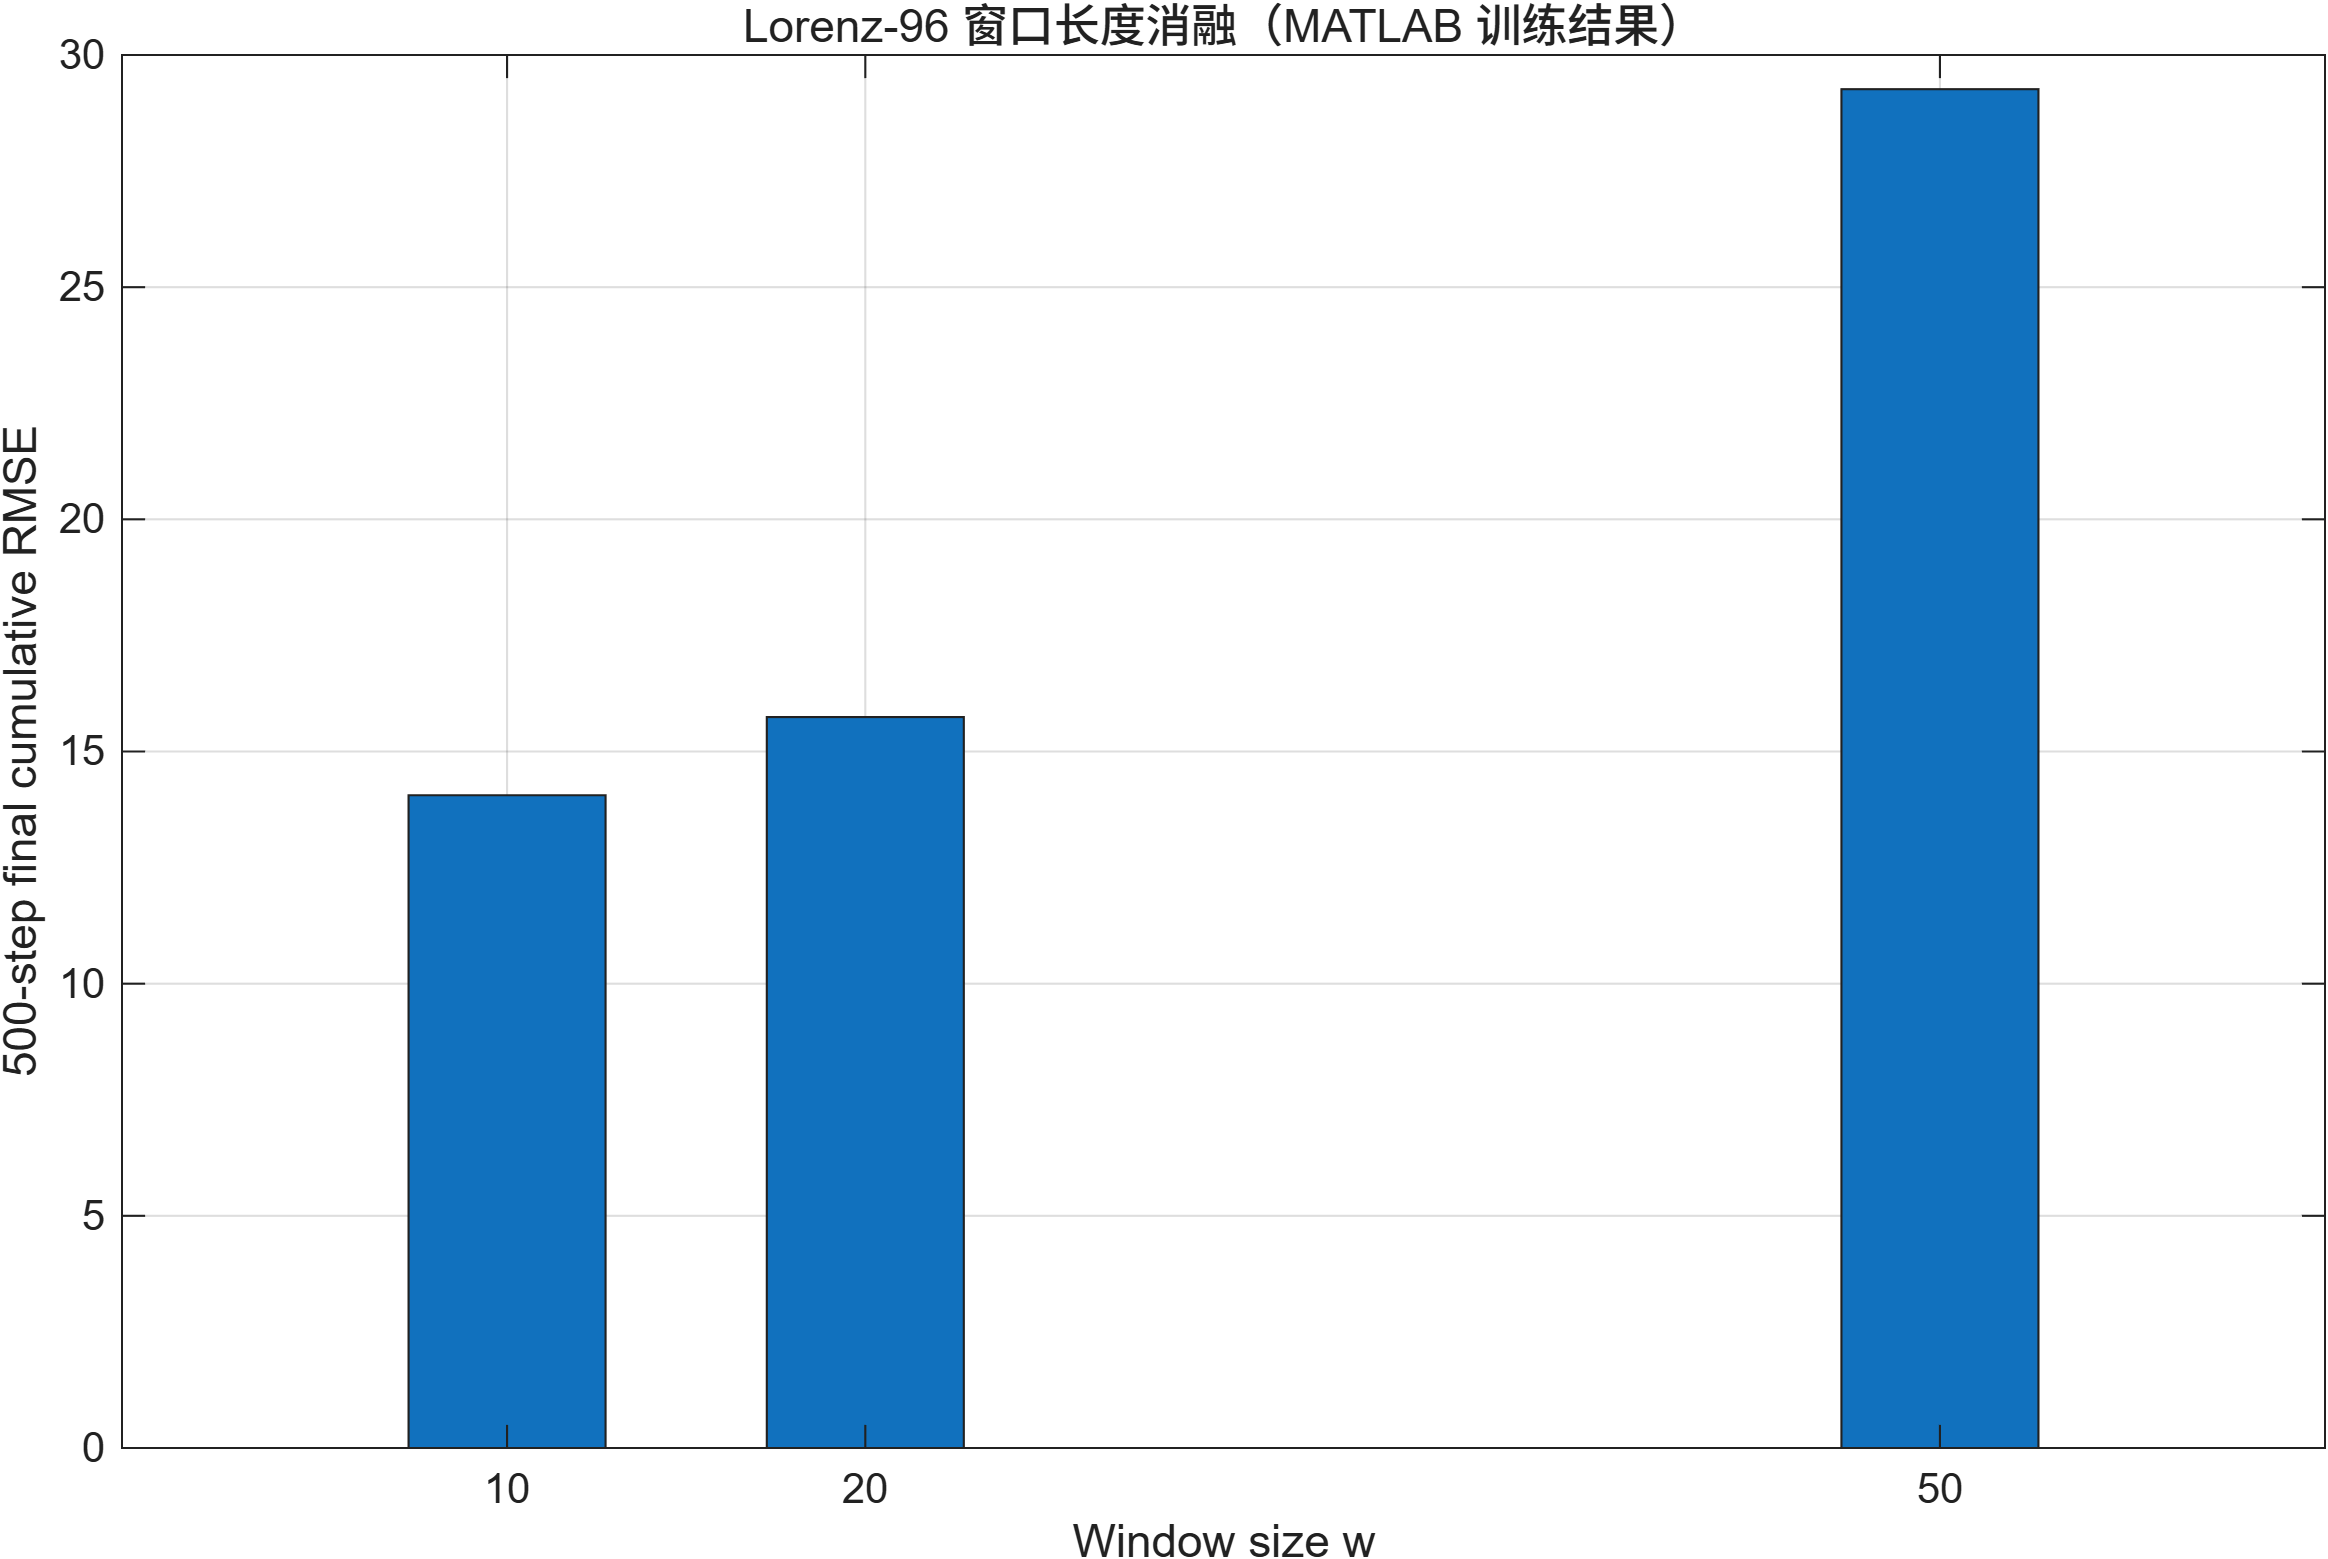
\includegraphics[width=\linewidth]{figures/lorenz96_window_ablation.png}
        \end{column}
    \end{columns}
\end{frame}

\begin{frame}{高级模型总体对比}
    \begin{columns}[T,onlytextwidth]
        \begin{column}{0.42\textwidth}
            \begin{table}
                \centering
                \small
                \begin{tabular}{lc}
                    \toprule
                    模型 & 500-step RMSE \\
                    \midrule
                    Baseline LSTM & 15.26 \\
                    PINN LSTM & 477.29 \\
                    Refined SS LSTM & 15.16 \\
                    Transformer & 23.25 \\
                    Hybrid LSTM & 78.42 \\
                    \textbf{Ultimate Hybrid} & \textbf{14.42} \\
                    \bottomrule
                \end{tabular}
            \end{table}
        \end{column}
        \begin{column}{0.56\textwidth}
            \centering
            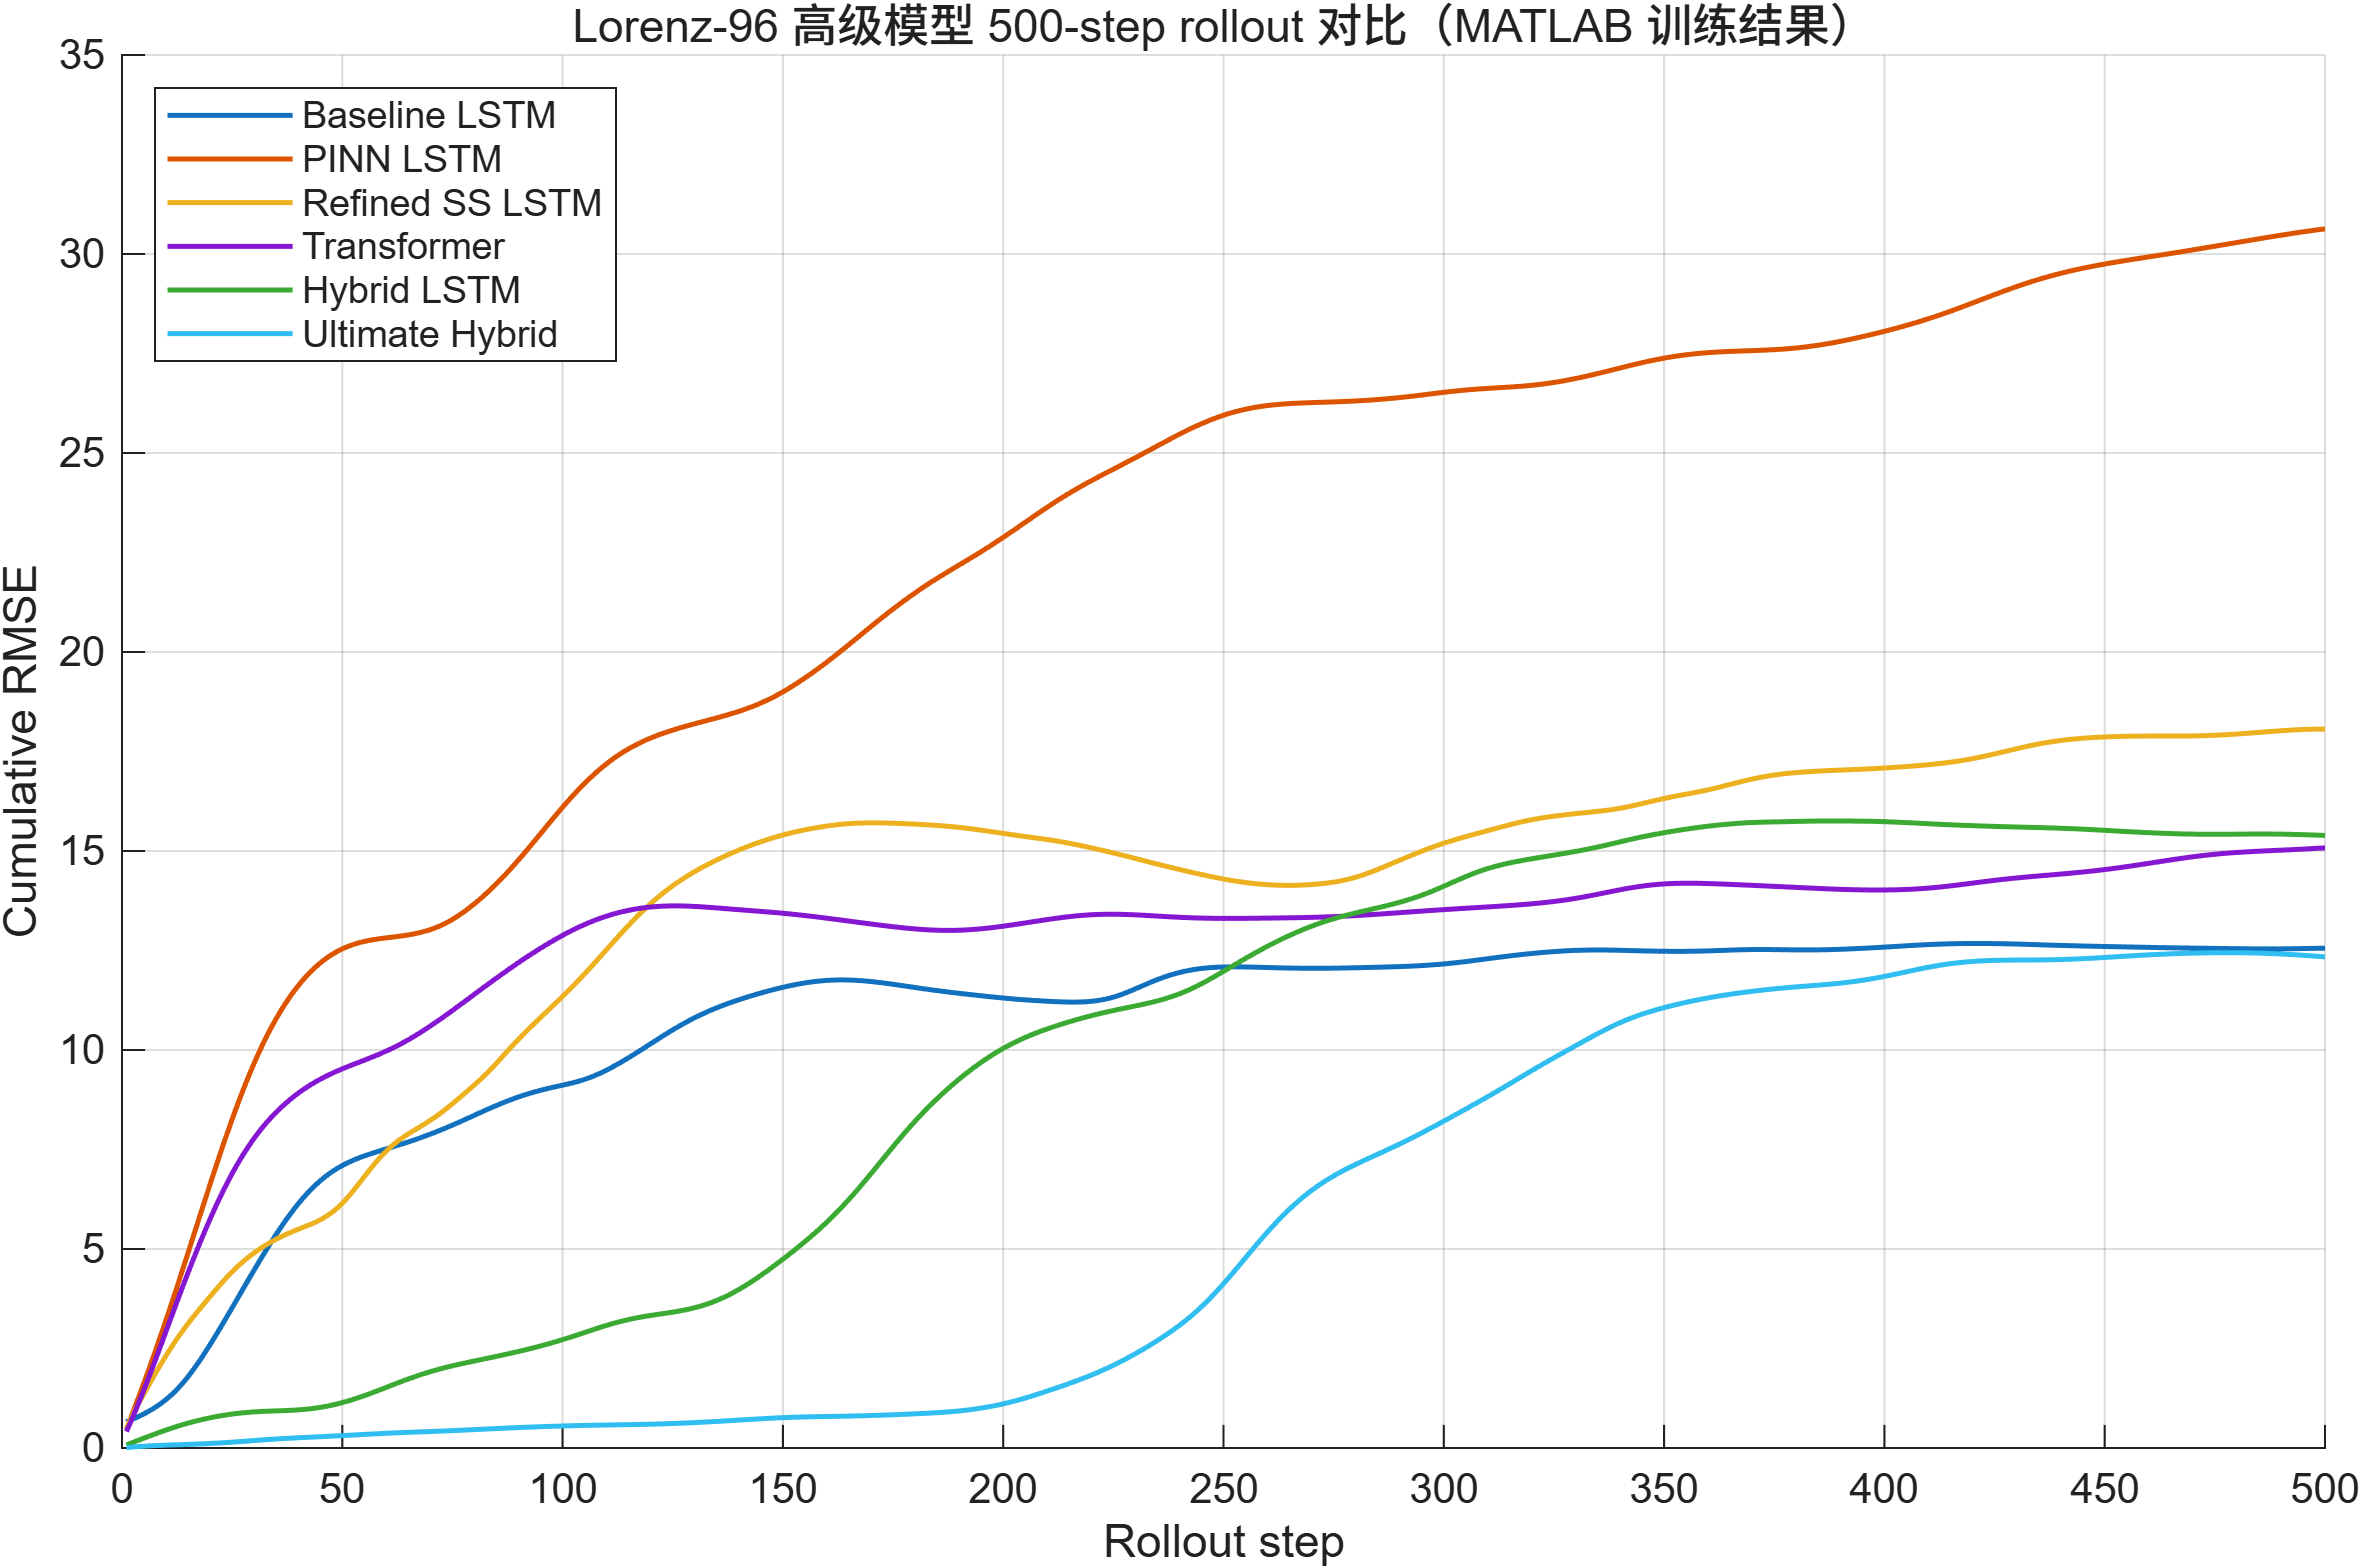
\includegraphics[width=\linewidth]{figures/lorenz96_advanced_rollout_comparison.png}
        \end{column}
    \end{columns}
\end{frame}

\begin{frame}{模块贡献分析}
    \begin{columns}[T,onlytextwidth]
        \begin{column}{0.48\textwidth}
            \begin{block}{物理约束}
                PINN 从动力学方程角度约束预测更新方向，使模型训练不只依赖数据误差。
            \end{block}
            \begin{block}{序列建模}
                Transformer 用 self-attention 提取历史窗口内的时间关联和相空间运动趋势。
            \end{block}
        \end{column}
        \begin{column}{0.48\textwidth}
            \begin{block}{物理基底}
                Hybrid physics 使用近似物理求解器提供基础演化，再由网络学习残差。
            \end{block}
            \begin{alertblock}{组合架构}
                Ultimate Hybrid 在当前 MATLAB 结果中达到 14.42，来自物理基底、残差模型、物理损失和多步训练的组合。
            \end{alertblock}
        \end{column}
    \end{columns}
\end{frame}

\begin{frame}{为什么 Ultimate Hybrid 最好？}
    \begin{enumerate}
        \item \textbf{物理基底降低漂移：} RK4 求解器给出合理的一步演化方向；
        \item \textbf{残差学习降低难度：} 神经网络只修正 $F_{\mathrm{imp}}=8.5$ 带来的系统偏差；
        \item \textbf{Transformer 利用历史：} self-attention 捕捉窗口中的相空间运动趋势；
        \item \textbf{PINN 保持动力学一致：} 限制预测更新不要明显违背 Lorenz-96 方程；
        \item \textbf{Scheduled sampling 贴近 rollout：} 训练阶段提前接触模型自身预测输入。
    \end{enumerate}
\end{frame}

\section{总结}

\begin{frame}{局限性}
    \begin{itemize}
        \item Lorenz-96 只测试 $N=10$、$F=8.0$，尚未覆盖更多维度和参数；
        \item 训练轮数统一为 20，未进行大规模超参数搜索；
        \item 当前结果主要来自单随机种子，缺少均值和方差；
        \item Ultimate Hybrid 还可继续做更细的 full ablation，例如 Transformer+PINN、Hybrid+PINN 等组合。
    \end{itemize}
\end{frame}

\begin{frame}{结论}
    \begin{enumerate}
        \item Lorenz-63 说明短期预测可学，但 recursive rollout 会迅速暴露长期误差累积；
        \item Lorenz-96 10D 的核心评价应是 500-step rollout，而不是 one-step RMSE；
        \item Residual learning、PINN、Transformer、Hybrid physics 和 scheduled sampling 从不同角度服务于长期稳定性建模；
        \item Ultimate Hybrid 在当前 MATLAB 结果中以 14.42 的最终累计 RMSE 取得最佳结果；
        \item 高维混沌预测更有效的路线是“物理模型作为基底，深度学习修正残差”。
    \end{enumerate}
\end{frame}

\begin{frame}[fragile]{代码演示与复现流程}
    \begin{block}{运行命令}
        \begin{verbatim}
matlab -batch "run_all_matlab"
matlab -batch "build_final_pdf"
        \end{verbatim}
    \end{block}
    \begin{block}{输出}
        \begin{itemize}
            \item \texttt{results/*.csv}
            \item \texttt{results/advanced/*.csv}
            \item \texttt{figures/*.png}
            \item \texttt{report.pdf}
        \end{itemize}
    \end{block}
\end{frame}

\end{document}
